%% !TEX program = xelatex
%% 中文 IEEE 格式稿。编译：xelatex Manuscript_FEE_Net_2026_zh.tex （跑两遍以生成交叉引用）
\documentclass[conference]{IEEEtran}
\usepackage{xeCJK}
\setmainfont{Times New Roman}
\setsansfont{Arial}
\setCJKmainfont[BoldFont=SimHei, ItalicFont=SimSun]{SimSun}
\setCJKsansfont[BoldFont=SimHei]{SimHei}
\setCJKmonofont{SimSun}
\newCJKfontfamily\heiti[BoldFont=SimHei]{SimHei}
\usepackage{amsmath,amssymb,amsfonts}
\usepackage{graphicx}
\usepackage{booktabs}
\usepackage{multirow}
\usepackage{url}
\usepackage{xcolor}
\usepackage{indentfirst}
\setlength{\parindent}{2em}

\renewcommand{\abstractname}{摘要}
\renewcommand{\IEEEkeywordsname}{关键词}
\renewcommand{\refname}{参考文献}
\renewcommand{\thesection}{\arabic{section}}
\renewcommand{\thesubsection}{\thesection.\arabic{subsection}}
\renewcommand{\tablename}{表}
\renewcommand{\figurename}{图}

% --- 会议版面压缩（EI 会议通常 6 页上限）---
\setlength{\textfloatsep}{8pt plus 2pt minus 2pt}
\setlength{\floatsep}{8pt plus 2pt minus 2pt}
\setlength{\intextsep}{8pt plus 2pt minus 2pt}
\setlength{\abovedisplayskip}{4pt plus 1pt minus 1pt}
\setlength{\belowdisplayskip}{4pt plus 1pt minus 1pt}
\renewcommand{\topfraction}{0.92}
\renewcommand{\bottomfraction}{0.70}
\renewcommand{\textfraction}{0.08}
\renewcommand{\floatpagefraction}{0.85}
\setcounter{topnumber}{3}
\setcounter{bottomnumber}{2}
\setcounter{totalnumber}{4}

\begin{document}

\title{频域边缘感知息肉分割网络的审计：组件级负结果与保形认证分流级联}

\author{\IEEEauthorblockN{医学人工智能研究团队}
\IEEEauthorblockA{（作者单位，院系）\\（城市 邮编，中国）\\（通信作者邮箱）}}

\maketitle

\begin{abstract}
\normalfont
结直肠癌是全球第三大常见恶性肿瘤、第二大癌症死因，而即便在专家操作下，结肠镜检查仍有约 17\%–28\% 的息肉被漏诊。深度分割模型在同一中心基准上报出的 Dice 已达 0.85–0.95，但跨中心部署时降至约 0.6–0.7；更关键的是，文献中报告的效率收益几乎都没有附带任何统计保证。本文认为，制约临床转化的瓶颈已不再是精度，而是“可保证性”：可审计的协议、可隔离的组件结论、可认证的工作点。为检验这一判断，我们在 Kvasir-SEG 的 150 例独立测试划分（训练开始前即已隔离）上，将一个频域边缘感知网络（FEE-Net，8.539 M 参数，12.59 GFLOPs）与三个同等训练的基线进行对照审计，得到三项结果。第一，该复合架构在 Dice 上并未超过朴素 U-Net（79.47\% 对 84.14\%），而参数量反而多 10.0\%。第二，组件归因推翻了原有设计依据，并揭示了该架构真正的价值所在：移除边缘门控模块后 Dice 升至 83.08\%（仅比 U-Net 低 1.06 个百分点），而 95\% 豪斯多夫距离降至 31.71 px，为全文最低——较 U-Net 的 36.33 px 降低 12.7\%，较最强基线 UNet++ 的 33.38 px 降低 5.0\%，即在重叠度基本持平的前提下取得显著更优的边界定位精度；三项辅助损失则均为正贡献（去深监督 -2.86、去边界 IoU -1.03、去边缘 BCE -0.63，联合 -2.95，且呈非可加性）。第三，仅在分布匹配、无泄漏队列上微调分流头的级联，取得校准阈值 $\tau$*=0.59、精确 Clopper–Pearson 上界 FNR $\le$ 3.92\%（95\% 置信）、在互不相交的认证集上实测漏诊 0/75、无病灶黏膜旁路率 99.25\%，实测延迟由 11.30 ms 降至 5.93 ms（1.91 倍）。此外我们记录了两个会静默失效的实现陷阱：在全部为阳性的队列上训练的分流头会坍缩为常数输出；冻结梯度并不能阻止批归一化统计量污染共享主干（Dice 由 81.42\% 跌至 14.06\%）。我们公开协议、单一真源基准生成器与溯源包，使上述结论可被重新推导，而不必被信任。
\end{abstract}

\begin{IEEEkeywords}
结肠镜息肉分割；离散小波变换；组件消融；保形风险控制；早退分流；无泄漏评测；可复现性
\end{IEEEkeywords}

\section{引言}

结直肠癌（CRC）是全球第三大常见恶性肿瘤与第二大癌症死因，预计到 2040 年全球新发病例将超过每年 320 万例\cite{divya2026review}。绝大多数 CRC 经由腺瘤—癌序列发生，因此在结肠镜下发现并完整切除癌前息肉，可在恶变之前阻断疾病进程\cite{divya2026review}。然而结肠镜是一项高度依赖操作者的检查：息肉形态差异极大，尤其直径小于 10 mm 的微小或平坦病变极易被忽略，文献报道即使由专家操作，仍有约 17\%–28\% 的息肉被漏诊\cite{xiao2026prysmnet}。

因此，深度学习已被广泛用于息肉的检测、分型与分割，并取得相当进展。2026 年的一篇系统综述梳理了该领域从 U 型卷积编码器向 Transformer 与状态空间主干演进的脉络，以及多尺度融合、注意力与合成数据等并行方向\cite{divya2026review}。在标准同中心基准上，现代分割模型的平均 Dice 通常落在 0.85–0.95 区间\cite{xiao2026prysmnet}。但这一数字对临床行为的预测力很弱。同一篇综述记录了模型在更换采集环境时出现 15.1\% 的泛化落差，并把实时性、不确定性估计与计算开销列为部署的主要障碍\cite{divya2026review}；2026 年发表于 npj Digital Medicine 的一项系统工作则把跨中心退化说得更直接：在 PolypGen 等未见数据集上，Dice 会跌至约 0.6–0.7\cite{xiao2026prysmnet}。可用来研究这一问题的资源同样不均衡：单中心数据集如 Kvasir-SEG 提供 1000 帧标注图像\cite{jha2020kvasir}，而 PolypGen 汇集 6 个中心、300 余例患者与 3446 个标注息肉，其建库目的正是评估泛化能力\cite{ali2023polypgen}。已发表模型绝大多数在前者上开发与验证。

当前研究主要沿三条架构路线展开，每条路线都带有在床旁场景中不可忽视的代价。Transformer 编码器通过自注意力建模全局上下文，但计算量随 token 数呈二次增长\cite{chen2021transunet}；以 Mamba 为代表的状态空间主干在保持长程建模能力的同时具有线性复杂度\cite{ruan2024vmunet}；可提示的基础模型具备广泛泛化能力，代价是大规模预训练与推理阶段的交互提示——例如 MedSAM 在 1 572 563 组图像—掩码对上训练，覆盖 10 种模态、30 余种癌症\cite{ma2024medsam}。上述路线都难以直接适用于算力受限条件下的逐帧筛查，这正是紧凑卷积设计在此类场景中仍有吸引力的原因。但这一选择通常仅以延迟作为论据，很少被逐组件审计。

在此背景下，我们识别出三个以精度为中心的汇报方式无法覆盖、却共同决定息肉分割器能否落地的方法学问题。

（一）协议泄漏与预算不可比。Kvasir-SEG 含 1000 帧标注图像\cite{jha2020kvasir}，而相当一部分文献在每次实验中重新随机划分。当测试帧是在超参数选择之后才被抽出，或基线训练的轮数少于所提模型时，所报差距就把架构效应与协议效应混在了一起。这一问题严重到 2026 年的一项系统工作明确指出：直到不久之前该领域都没有标准化的跨域评测协议，因此许多论文只报告同中心指标，而这些指标“并不能保证真实世界的临床可靠性”\cite{xiao2026prysmnet}。

（二）组件结论未被隔离。息肉分割架构通常把一个小波前端、一个通道注意力模块、一个方向滤波器和若干辅助损失打包在一起，然后把总体增益归因于整个组合。由于小波引导与边缘引导的息肉分割已是拥挤的研究方向——离散小波下采样\cite{zhao2023wranet}、小波与注意力 U-Net 结合\cite{rajasekar2024adaptunet}、免参数 Haar 边缘注入\cite{yeemeganet2025}、小波跨频带融合\cite{oh2026crossband}——任何新组合的边际价值只能通过在固定预算下逐项移除来确立。

（三）效率与安全声明缺乏保证。常规筛查的绝大部分视帧是非病理性黏膜，因此跳过明显阴性的帧是回收延迟的自然思路。早退网络按样本在运行时裁剪计算深度\cite{laskaridis2021earlyexit}，在分类基准上基于全局平均池化的出口已能在显著降低计算量的同时保持与非早退版本相当的精度\cite{demir2024earlyexit}。但决定“跳过”的阈值本质上是一条临床决策规则，而一条通过检视自身测试表现来选定的规则，不提供任何保证。

分布无关风险控制恰好提供了缺失的那一环：风险控制预测集可对一般损失给出有限样本保证\cite{bates2021rcps}，保形风险控制把这一保证推广到任意单调损失\cite{angelopoulos2022crc}，而分裂保形的有效性依赖校准集与测试集之间的可交换性\cite{angelopoulos2021gentle}。医学影像领域已开始把这些工具用于病灶分割\cite{tan2025cls,dai2025crcfdr}，而 2026 年的一项研究给出了必要的警示：在 PET/CT 肿瘤分割中，二值漏诊损失在 $\alpha$=$\delta$=0.1 下无法被认证，因为即便取所评估的最小阈值，校准集上的经验风险仍为 0.177——作者正确地将其诊断为预测族的支撑失败，而非保形风险控制本身的失败\cite{zheng2026crc}。

本文对一个正是围绕上述三个假设设计的频域边缘感知网络（FEE-Net）进行审计。我们不以“架构成功”的方式呈现它，而是把它置于可审计的标准之下，报告哪些部分经受住了检验。本文的贡献有四项。

\begin{enumerate}
  \item 无泄漏、单一真源的基准。150 例测试划分在训练前即被隔离，并由程序化的不相交断言强制执行；产出全部数字的流程把仓库中的模型与损失源码逐字内联，作为包导入，断言每个类都解析到内联副本，并把该副本与划分文件一并封入结果包作为溯源产物。
  \item 含负结果的组件级归因。在单一随机种子、单一划分与统一 60 轮预算下，我们隔离了三项辅助损失（深监督、边界 IoU、边缘 BCE）与两个架构分支（小波前端、边缘门控模块）。三项辅助损失各自有益且联合呈次可加；边缘门控模块在 Dice 与边界误差上均有害，该族的最佳配置是移除该模块的变体。需要强调的是，该变体在 95\% 豪斯多夫距离上取得 31.71 px 的全场最优值，较 U-Net 降低 12.7\%、较 UNet++ 降低 5.0\%，说明频域与边界监督的收益主要体现在边界定位而非区域重叠。
  \item 保形认证的分流级联。在由留出帧构建的无泄漏混合队列上，且校准与认证严格分离，我们得到 $\tau$*=0.59、认证漏诊率 0/75、95\% 置信下精确 Clopper–Pearson 上界 3.92\%、无病灶黏膜旁路率 99.25\%，以及实测 1.91 倍的延迟下降。我们同时报告实测率与其上界，这是保形文献的要求。
  \item 两个可推广的失效模式。在全部为阳性的队列上训练的分流头会坍缩为常数输出；仅微调分流头而让共享主干停留在训练模式的方案，会静默改写其批归一化统计量，使分割 Dice 从 81.42\% 跌至 14.06\%。两者对损失曲线均不可见，我们给出纠正配方。
\end{enumerate}

我们明确说明不主张什么。我们不主张达到最先进 Dice；恰恰相反，本文主要的分割结论是负面的，第6.2 节解释了为何该文献中的已发表数字与本文不可直接比较。我们所主张的是：协议、归因与认证三者可从公开产物重新推导，而这一组合对部署的贡献大于再提高零点几个 Dice 点。

\section{相关工作}

\subsection{息肉与医学图像分割}

U-Net 以带跳跃连接的编码器—解码器确立了生物医学分割的基本范式\cite{ronneberger2015unet}。UNet++ 引入嵌套稠密跳跃路径以缩小编码器与解码器特征之间的语义差距，并采用深监督\cite{zhou2018unetpp}；Attention U-Net 以加性注意力门抑制无关区域、突出与任务相关的显著特征\cite{oktay2018attention}。Transformer 路线以 TransUNet 为代表，用自注意力提取全局上下文\cite{chen2021transunet}；Mamba 路线以 VM-UNet 为代表，在保持长程建模的同时避免二次复杂度\cite{ruan2024vmunet}；基础模型路线以 MedSAM 为代表，强调跨模态的通用分割能力\cite{ma2024medsam}。专门面向息肉的方法中，PraNet 以并行部分解码器聚合高层特征、以反向注意力挖掘边界线索，在 Kvasir 上报告 0.898 Dice\cite{fan2020pranet}。本文与上述工作的关系是补充而非竞争：我们关注的是系统级的筛查效率与可认证性，并在同一协议下审计一个紧凑卷积设计。

\subsection{频域表示与小波}

频域方法把图像信号分解为全局结构趋势与局部梯度跃变。傅里叶变换缺乏空间定位，而离散小波变换（DWT）在无混叠的前提下提供联合的时频定位。在息肉分割中，小波已是一条成熟路线：WRANet 以 DWT 取代最大/平均池化，分解后去除高频分量以抑制噪声，并在 CVC-ClinicDB 上报告 88.89\% Dice\cite{zhao2023wranet}；AdaptUNet 把小波前端与注意力 U-Net 结合，在 HyperKvasir 上训练后于 CVC-300 报告 0.9104 Dice\cite{rajasekar2024adaptunet}；MEGANet-W 把免参数的 Haar 小波边缘图注入每个解码器阶段，在五个息肉数据集上最高提升 1.2 mDice\cite{yeemeganet2025}；2026 年的跨频带框架通过融合 RGB 与灰度的小波子带，在 Kvasir 上报告 0.885 mDice，其论据是灰度表示在各细节频带上保持了更高的边界对比度\cite{oh2026crossband}。就通道注意力而言，压缩—激励结构确立了按通道重标定的有效性\cite{hu2018senet}；FcaNet 进一步证明全局平均池化本身只是频域特征分解的一个特例，保留多个频率分量可以得到比单一池化更丰富的通道描述子\cite{qin2021fcanet}。

\subsection{边界感知损失}

边界监督研究充分。Karimi 与 Salcudean 通过对真值预测差异图施加形态学腐蚀来直接优化豪斯多夫距离\cite{karimi2019hd}；El Jurdi 等提出以最大池化膨胀减去最小池化腐蚀得到的软轮廓来约束周长\cite{eljurdi2021perimeter}；同一带状构造也是 Boundary IoU 这一边界质量度量的基础\cite{cheng2021boundaryiou}。Dice 目标最早被用于应对前景—背景体素的强烈不平衡\cite{milletari2016vnet}，深监督则源自为中间层附加“伴随目标”的构造\cite{lee2015dsn}。本文的复合损失采用上述既有算子，贡献不在算子本身，而在把它们纳入息肉流水线后的逐项归因。

\subsection{保形风险控制与动态推理}

动态推理通过让简单样本提前退出降低平均延迟，但朴素的置信度阈值不提供任何统计保证——当一次假阴性意味着漏掉一个肿瘤时，这是不可接受的。风险控制预测集可对一般损失给出分布无关的有限样本控制\cite{bates2021rcps}，保形风险控制把这一框架推广到任意单调损失，且保守性至多差 O(1/n)\cite{angelopoulos2022crc}；分裂保形在可交换性假设下给出覆盖保证\cite{angelopoulos2021gentle}。医学应用推进很快：CLS 为每例扫描校准阈值，使测试期假阴性率低于给定容差\cite{tan2025cls}；保形风险控制也被用于管理医学实例分割中的错误发现率\cite{dai2025crcfdr}。两条警示塑造了我们的协议：校准与评测必须使用可交换但互不相交的样本；对二值漏诊损失，在严格风险水平下认证可能根本不可行\cite{zheng2026crc}。因此我们在验证折上校准 $\tau$*，在留出测试集上仅认证一次，并同时报告实测率与精确上界。

\section{方法}

\subsection{总体架构}

给定输入 X $\in$ $\mathbb{R}$\textsuperscript{3$\times$H$\times$W}（H = W = 256），FEE-Net 由以下部分构成：（i）残差多尺度编码器，输出 e\textsubscript{1} 至 e\textsubscript{4}；（ii）两级二维 Haar DWT 与谱通道注意力（SCA），提取经眩光纯化的高频特征；（iii）空洞残差瓶颈与双线性上采样解码器（避免转置卷积的棋盘伪影\cite{odena2016checker}）；（iv）在最细两个尺度上以全向小波滤波（ODWF）融合纯化边缘与解码语义的边缘门控模块（EGM）；（v）多尺度深监督头；（vi）共享主干的早退分流头，其阈值 $\tau$* 由保形方法校准。完整分割路径由复合损失监督（第3.4 节），分流头以停止梯度探针训练（第3.5 节）。

\subsection{二维 Haar 小波与谱通道注意力}

二维 Haar DWT 把特征图 F $\in$ $\mathbb{R}$\textsuperscript{C$\times$H$\times$W} 分解为四个空间下采样的子带：

\begin{align}
\mathbf{F}_{LL} &= (\mathbf{F}_{00}+\mathbf{F}_{01}+\mathbf{F}_{10}+\mathbf{F}_{11})/2\\\mathbf{F}_{LH} &= (-\mathbf{F}_{00}-\mathbf{F}_{01}+\mathbf{F}_{10}+\mathbf{F}_{11})/2\\\mathbf{F}_{HL} &= (-\mathbf{F}_{00}+\mathbf{F}_{01}-\mathbf{F}_{10}+\mathbf{F}_{11})/2\\\mathbf{F}_{HH} &= (\mathbf{F}_{00}-\mathbf{F}_{01}-\mathbf{F}_{10}+\mathbf{F}_{11})/2
\end{align}

其中 F\textsubscript{ij} = F[:, :, i::2, j::2]。该变换是正交的，因此高频信息在被解码器选择性复用之前并未被破坏。

原始子带把真实的边界能量与腔道液体产生的镜面眩光混在一起。通道注意力惯例上先以全局平均池化压缩特征，再做重标定，压缩—激励结构已证明这种重标定有效\cite{hu2018senet}；FcaNet 随后指出全局平均池化本身是频域分解的特例，保留多个频率分量可得更丰富的通道描述子\cite{qin2021fcanet}。本文模块以另一条路径得到同样结论：由于它本就作用于小波细节子带，其描述子是在频域中天然构成的，而不是从空间特征图恢复出来的。拼接后的细节张量 F\textsubscript{cat} = [F\textsubscript{LH} $\|$ F\textsubscript{HL} $\|$ F\textsubscript{HH}] 经双池化重标定：

\begin{equation}
\small
\begin{aligned}\mathbf{a}=\sigma\!\Big(&\mathbf{W}_2\,\mathrm{ReLU}(\mathbf{W}_1\,\mathrm{GAP}(\mathbf{F}_{cat}))\\&+\mathbf{W}_2\,\mathrm{ReLU}(\mathbf{W}_1\,\mathrm{GMP}(\mathbf{F}_{cat}))\Big)\end{aligned}
\end{equation}

其中 W\textsubscript{1} $\in$ $\mathbb{R}$\textsuperscript{3C/r$\times$3C}、W\textsubscript{2} $\in$ $\mathbb{R}$\textsuperscript{3C$\times$3C/r}，压缩比 r = 8，$\sigma$ 为 sigmoid。纯化特征为

\begin{equation}
\mathbf{F}_{hf}=\mathrm{Conv}_{1\times1}(\mathbf{F}_{cat}\odot\mathbf{a})
\end{equation}

此处保留全局最大池化是必要的：眩光占据小而亮的区域，其统计量在平均池化下会被抹平。

\subsection{全向小波滤波边缘门控模块}

方形 3$\times$3 卷积核存在方向偏置，会欠检测平坦息肉典型的 45°/135° 浸润前缘。因此 EGM 在（已调整尺寸的）频率特征上叠加三个互补的深度可分离核：

\begin{equation}
\small
\begin{aligned}\mathbf{F}_{dir}=\mathrm{ReLU}\Big(&\mathcal{K}_{1\times3}(\mathbf{F}_{freq})+\mathcal{K}_{3\times1}(\mathbf{F}_{freq})\\&+\mathcal{K}_{3\times3}^{diag}(\mathbf{F}_{freq})\Big)\end{aligned}
\end{equation}

为防止高频噪声污染语义区域，一个由受监督的粗预测 P\textsubscript{coarse} 调制的语义置信门对方向响应进行滤波：

\begin{equation}
\small
\begin{aligned}\mathbf{F}_{pure}=\mathbf{F}_{dir}\odot\Big[&\sigma\big(\mathrm{Conv}_{1\times1}(\mathrm{ReLU}(\mathrm{BN}(\mathrm{Conv}(\mathbf{F}_{dec}))))\big)\\&\odot\mathcal{U}(\sigma(\mathbf{P}_{coarse}))\Big]\end{aligned}
\end{equation}

随后以跨模态亲和图与可学习残差阻尼因子 $\gamma$（初值 0.1）把结果融合进解码器。该模块即表2中“w/o EGM”各行所移除的对象。

\subsection{复合损失与深监督}

分割路径由下式监督：

\begin{equation}
\small
\begin{aligned}\mathcal{L}=&\lambda_{bce}\mathcal{L}_{BCE}+\lambda_{dice}\mathcal{L}_{Dice}+\lambda_{b}\mathcal{L}_{BoundIoU}\\&+\lambda_{e}\mathcal{L}_{edge}+\lambda_{ds}\mathcal{L}_{ds}\end{aligned}
\end{equation}

其中 $\lambda$\textsubscript{bce} = $\lambda$\textsubscript{dice} = 1，$\lambda$\textsubscript{b} = 0.1，$\lambda$\textsubscript{e} = 0.2，$\lambda$\textsubscript{ds} = 0.3。Dice 项沿用为应对强烈前景—背景不平衡而提出的目标\cite{milletari2016vnet}，深监督项沿用为中间表示附加伴随目标、而非仅在输出端施加损失的构造\cite{lee2015dsn}。L\textsubscript{BoundIoU} 使用厚度 d = 3 的形态学带状区域，由最大池化膨胀减最小池化腐蚀得到\cite{eljurdi2021perimeter,karimi2019hd}，并以其可微的 Boundary-IoU 形式求值\cite{cheng2021boundaryiou}。L\textsubscript{edge} 是施加于辅助边缘头的 BCE 项；L\textsubscript{ds} 在把三个深监督输出双线性缩放至目标分辨率后取同一准则的平均。解码器使用双线性上采样而非转置卷积，依据的是关于棋盘伪影的分析\cite{odena2016checker}。

\subsection{共享主干分流头与两阶段训练}

分流头读取第一编码阶段与第一级纯化小波特征。由于微小息肉所占像素比例可以忽略，标准早退模块所用的全局平均池化描述子会稀释其激活\cite{demir2024earlyexit}；因此我们构造四分支描述子

\begin{equation}
\small
\begin{aligned}\mathbf{z}=[&\mathrm{GAP}(\mathbf{e}_1)\|\mathrm{GMP}(\mathbf{e}_1)\\&\|\mathrm{GAP}(\mathbf{F}_{hf}^{1})\|\mathrm{GMP}(\mathbf{F}_{hf}^{1})]\in\mathbb{R}^{4C}\end{aligned}
\end{equation}

并以停止梯度探针分类：$\hat{y}$\textsubscript{risk} = Softmax(MLP(sg(z)))\textsubscript{1}，使该辅助目标无法重塑分割表示。

训练分两阶段。第一阶段在 fold-0 训练划分上以复合损失训练主干。第二阶段仅优化分流头（12 740 个参数），数据为用同一裁剪流程从 fold-0 训练与验证帧构建的均衡队列，使其输入分布与部署一致：含小病灶的完整帧与黏膜裁剪。第二阶段令共享路径保持推理模式，仅分流头处于训练模式。该阶段不修改主干，训练后我们核验分割 Dice 保持在 81.42\% 不变。

\subsection{保形风险控制}

设校准集 D\textsubscript{cal} = {(X\textsubscript{i}, Y\textsubscript{i} = 1)}\textsubscript{i=1}\textsuperscript{n} 为真实息肉帧。对阈值 $\tau$，当 $\hat{y}$\textsubscript{risk} < $\tau$ 时该帧被旁路，漏诊数为 k($\tau$) = $\Sigma$\textsubscript{i} 1($\hat{y}$\textsubscript{risk}(X\textsubscript{i}) < $\tau$)。精确上置信界为

\begin{equation}
U_{1-\delta}(\tau)=\mathrm{BetaInv}\!\left(1-\delta;\,k(\tau)+1,\,n-k(\tau)\right)
\end{equation}

当 k = 0 时该式退化为 1 - $\delta$\textsuperscript{1/n}\cite{clopper1934}。我们选取

\begin{equation}
\tau^{*}=\max\{\tau:\ U_{1-\delta}(\tau)\le\alpha\}
\end{equation}

其中 $\alpha$ = 0.05、$\delta$ = 0.05，随后在互不相交的认证半集上一次性认证，同时报告经验率与其上界。当 n = 75、k = 0 时上界为 1 - 0.05\textsuperscript{1/75} = 3.92\%，我们以该闭式作为实现的单元校验。

\section{实验设置}

\subsection{数据与无泄漏划分}

Kvasir-SEG 提供 1000 帧内镜图像及二值息肉掩码，由一名工程师与一名医生勾画、经经验丰富的消化内科医师复核\cite{jha2020kvasir}。全部帧缩放至 256$\times$256；图像转 RGB 并归一化到 [0,1]，掩码以灰度 127 为阈值二值化后以最近邻重采样。当掩码像素数超过 10 时，该帧标记为病灶阳性，该阈值用于排除标注噪点。

划分固定并随仓库发布：680 帧训练、170 帧验证、150 帧测试，按病灶面积分层。流程在运行时断言三者两两不相交，一旦违反即中止运行。测试划分不用于任何形式的模型选择。

\subsection{混合筛查队列}

由于源数据集全部为阳性，我们从 150 帧留出测试帧构建混合队列。对每一帧，阳性样本即该帧本身；阴性样本为同一帧中的方形黏膜裁剪，要求距标注掩码至少 20 像素、边长不小于 64 像素，在掩码补集的距离变换局部极大处选取，并排除暗边框像素；每帧最多取两处。裁剪缩放至 256$\times$256，配以全零掩码。

队列按排序后帧列表的序号交替划分，使任一帧不会同时进入两半：校准半含 75 例病灶与 134 例黏膜裁剪，认证半含 75 例病灶与 133 例黏膜裁剪。以帧而非样本为不相交单位是必要的，因为同帧裁剪共享光照与光学条件。

\subsection{训练协议与测量}

所有模型训练 60 轮，优化器为 Adam，批大小 16，初始学习率 10\textsuperscript{-4} 并采用余弦衰减，输入分辨率 256$\times$256。60 轮预算在审计开始前即已固定，依据是一次收敛检查：复合损失在 35 轮时仍在改善（验证 Dice 76.14\%），到 60 轮趋于平台（77.55\%）。该决策未使用任何测试划分信息。

FLOPs 由 ThOP 在 256$\times$256、批大小为 1 下统计。延迟与 FPS 在单台设备上经预热后以非阻塞 CUDA 事件对重复单帧前向测量；对早退模型，测量时以包装器强制走完整分割路径，而非分流门。绝对延迟与设备相关，按此如实报告。

\subsection{评价指标}

Dice、平均 IoU、精确率与召回率在 0.5 阈值二值化后计算。HD95 取对称表面距离的 95 分位数，在工作分辨率 256$\times$256 下统计。我们以像素报告 HD95 而不换算为毫米：源帧存在多种原始分辨率，单一像素—毫米系数会产生误导。

\subsection{可复现性与溯源}

基准由单一脚本生成：该脚本把仓库中的模型、损失与指标源码逐字内联进流程，在运行时物化为一个包，并断言每个被导入的类都解析到该物化副本而非陈旧的安装。同一结果包内含划分文件、实测参数量/FLOPs/延迟表与逐样本风险分数 CSV，使认证结果可被独立重算。本文每一个数字都对应上述产物之一，映射关系见随附的参考文献与产物清单。

\section{结果}

\subsection{基准完整性与队列构成}

本次审计运行于 Kvasir-SEG。训练前我们固定了单一分层划分：680 帧训练、170 帧验证、150 帧作为独立测试划分（表1）。测试划分在训练与模型选择中从不被触及，流程在运行时断言三集合两两不相交，一旦违反即中止而非告警。

\begin{table}[t]
\centering

\caption{表1 本研究使用的数据划分。测试划分在训练前隔离；混合筛查队列仅由留出测试帧派生，并按排序序号交替拆分为互不相交的校准半与认证半。}
\label{tab:partitions}
\resizebox{\columnwidth}{!}{%
\begin{tabular}{lcc}
\toprule
\textbf{角色} & \textbf{来源} & \textbf{帧数} \\
\midrule
训练 & Kvasir-SEG，fold 0 & 680 \\
验证（模型选择） & Kvasir-SEG，fold 0 & 170 \\
独立测试 & Kvasir-SEG，留出 & 150 \\
混合队列·校准 & 测试帧，病灶 & 75 \\
 & 测试帧，黏膜裁剪 & 134 \\
混合队列·认证 & 测试帧，病灶 & 75 \\
 & 测试帧，黏膜裁剪 & 133 \\
\bottomrule
\end{tabular}}
\end{table}

该设计有两点对解读至关重要。第一，表2中每个模型看到的都是同一 680/170 划分、同一增强、同一 60 轮预算与同一损失族，因此行间差异可归因于架构而非训练日程。第二，所有数值均为固定种子下的单次点估计。我们在第6.4 节回到这一限制；也正因如此，我们把本基准称为审计，而非排行榜条目。

\subsection{分割精度：复合架构未超过朴素 U-Net}

表2给出 150 例留出测试集的结果。由该表可直接得到三点观察。

\begin{table*}[t]
\centering
\footnotesize
\caption{表2 150 帧独立测试划分上的分割性能。所有行共享同一划分、增强、60 轮预算与损失族；数值为固定种子下的单次点估计。FLOPs 为 256$\times$256、批大小 1 下的 ThOP 统计；延迟与 FPS 为单台设备上的 CUDA 事件测量（第4.3 节）。加粗为各列最优。}
\label{tab:main}
\resizebox{\textwidth}{!}{%
\begin{tabular}{lccccccccc}
\toprule
\textbf{模型} & \textbf{Dice (\%)↑} & \textbf{mIoU (\%)↑} & \textbf{HD95 (px)↓} & \textbf{精确率 (\%)↑} & \textbf{召回率 (\%)↑} & \textbf{参数量 (M)} & \textbf{FLOPs (G)↓} & \textbf{延迟 (ms)↓} & \textbf{FPS↑} \\
\midrule
U-Net \cite{ronneberger2015unet} & 84.14 & 76.45 & 36.33 & 89.34 & 82.60 & 7.763 & 13.75 & 10.02 & 99.8 \\
Attention U-Net \cite{oktay2018attention} & 84.00 & 75.83 & 38.73 & 90.21 & 81.43 & 7.852 & 14.03 & 11.57 & 86.5 \\
UNet++ \cite{zhou2018unetpp} & 84.07 & 76.57 & 33.38 & 89.67 & 83.23 & 9.160 & 34.62 & 16.92 & 59.1 \\
FEE-Net & 79.47 & 70.65 & 38.67 & 86.55 & 75.33 & 8.539 & 12.59 & 15.66 & 63.9 \\
FEE-Net-EE & 81.42 & 73.07 & 36.41 & 86.26 & 78.90 & 8.552 & 12.59 & 17.43 & 57.4 \\
FEE-Net w/o DWT & 80.78 & 72.73 & 36.11 & 86.83 & 80.19 & 8.546 & 12.87 & 14.35 & 69.7 \\
FEE-Net w/o EGM & 83.08 & 75.59 & 31.71 & 87.84 & 82.92 & 8.522 & 11.83 & 11.94 & 83.8 \\
\bottomrule
\end{tabular}}
\end{table*}

第一，三个经典基线在 Dice 上彼此难以区分（84.14\%、84.00\%、84.07\%），而计算量相差 2.5 倍（13.75、14.03、34.62 GFLOPs）。在匹配预算下，UNet++ 多出的容量并未在重叠度上换来任何收益。

第二，FEE-Net 的 Dice 为 79.47\%，比 U-Net 低 4.67 个百分点，是表中最低值。其参数量为 8.539 M，比 U-Net 的 7.763 M 多 10.0\%；计算量为 12.59 GFLOPs，比 U-Net 少 8.4\%、比 UNet++ 少 63.6\%。可见该架构在计算轴上确实占据了一个位置，但在精度轴上付出了代价。图\ref{fig:pareto} 把七种配置置于精度—计算平面上，其中并无支配者：基线以 13.75–34.62 GFLOPs 换取精度，而所提族的消融变体以 11.83 GFLOPs 位于其下。FEE-Net 的精确率（86.55\%）与召回率（75.33\%）均低于所有基线，在定性结果上表现为小的假阳卫星区域以及病灶本体的欠分割（图\ref{fig:qual}）。

第三，早退变体 FEE-Net-EE 达到 81.42\% Dice、73.07\% mIoU 与 36.41 px HD95，计算量同为 12.59 GFLOPs，回收了部分差距。我们的设计未隔离该回收的成因，故仅作为观察报告，而不作为机制证据；它不改变排序。

\begin{figure*}[t]
\centering
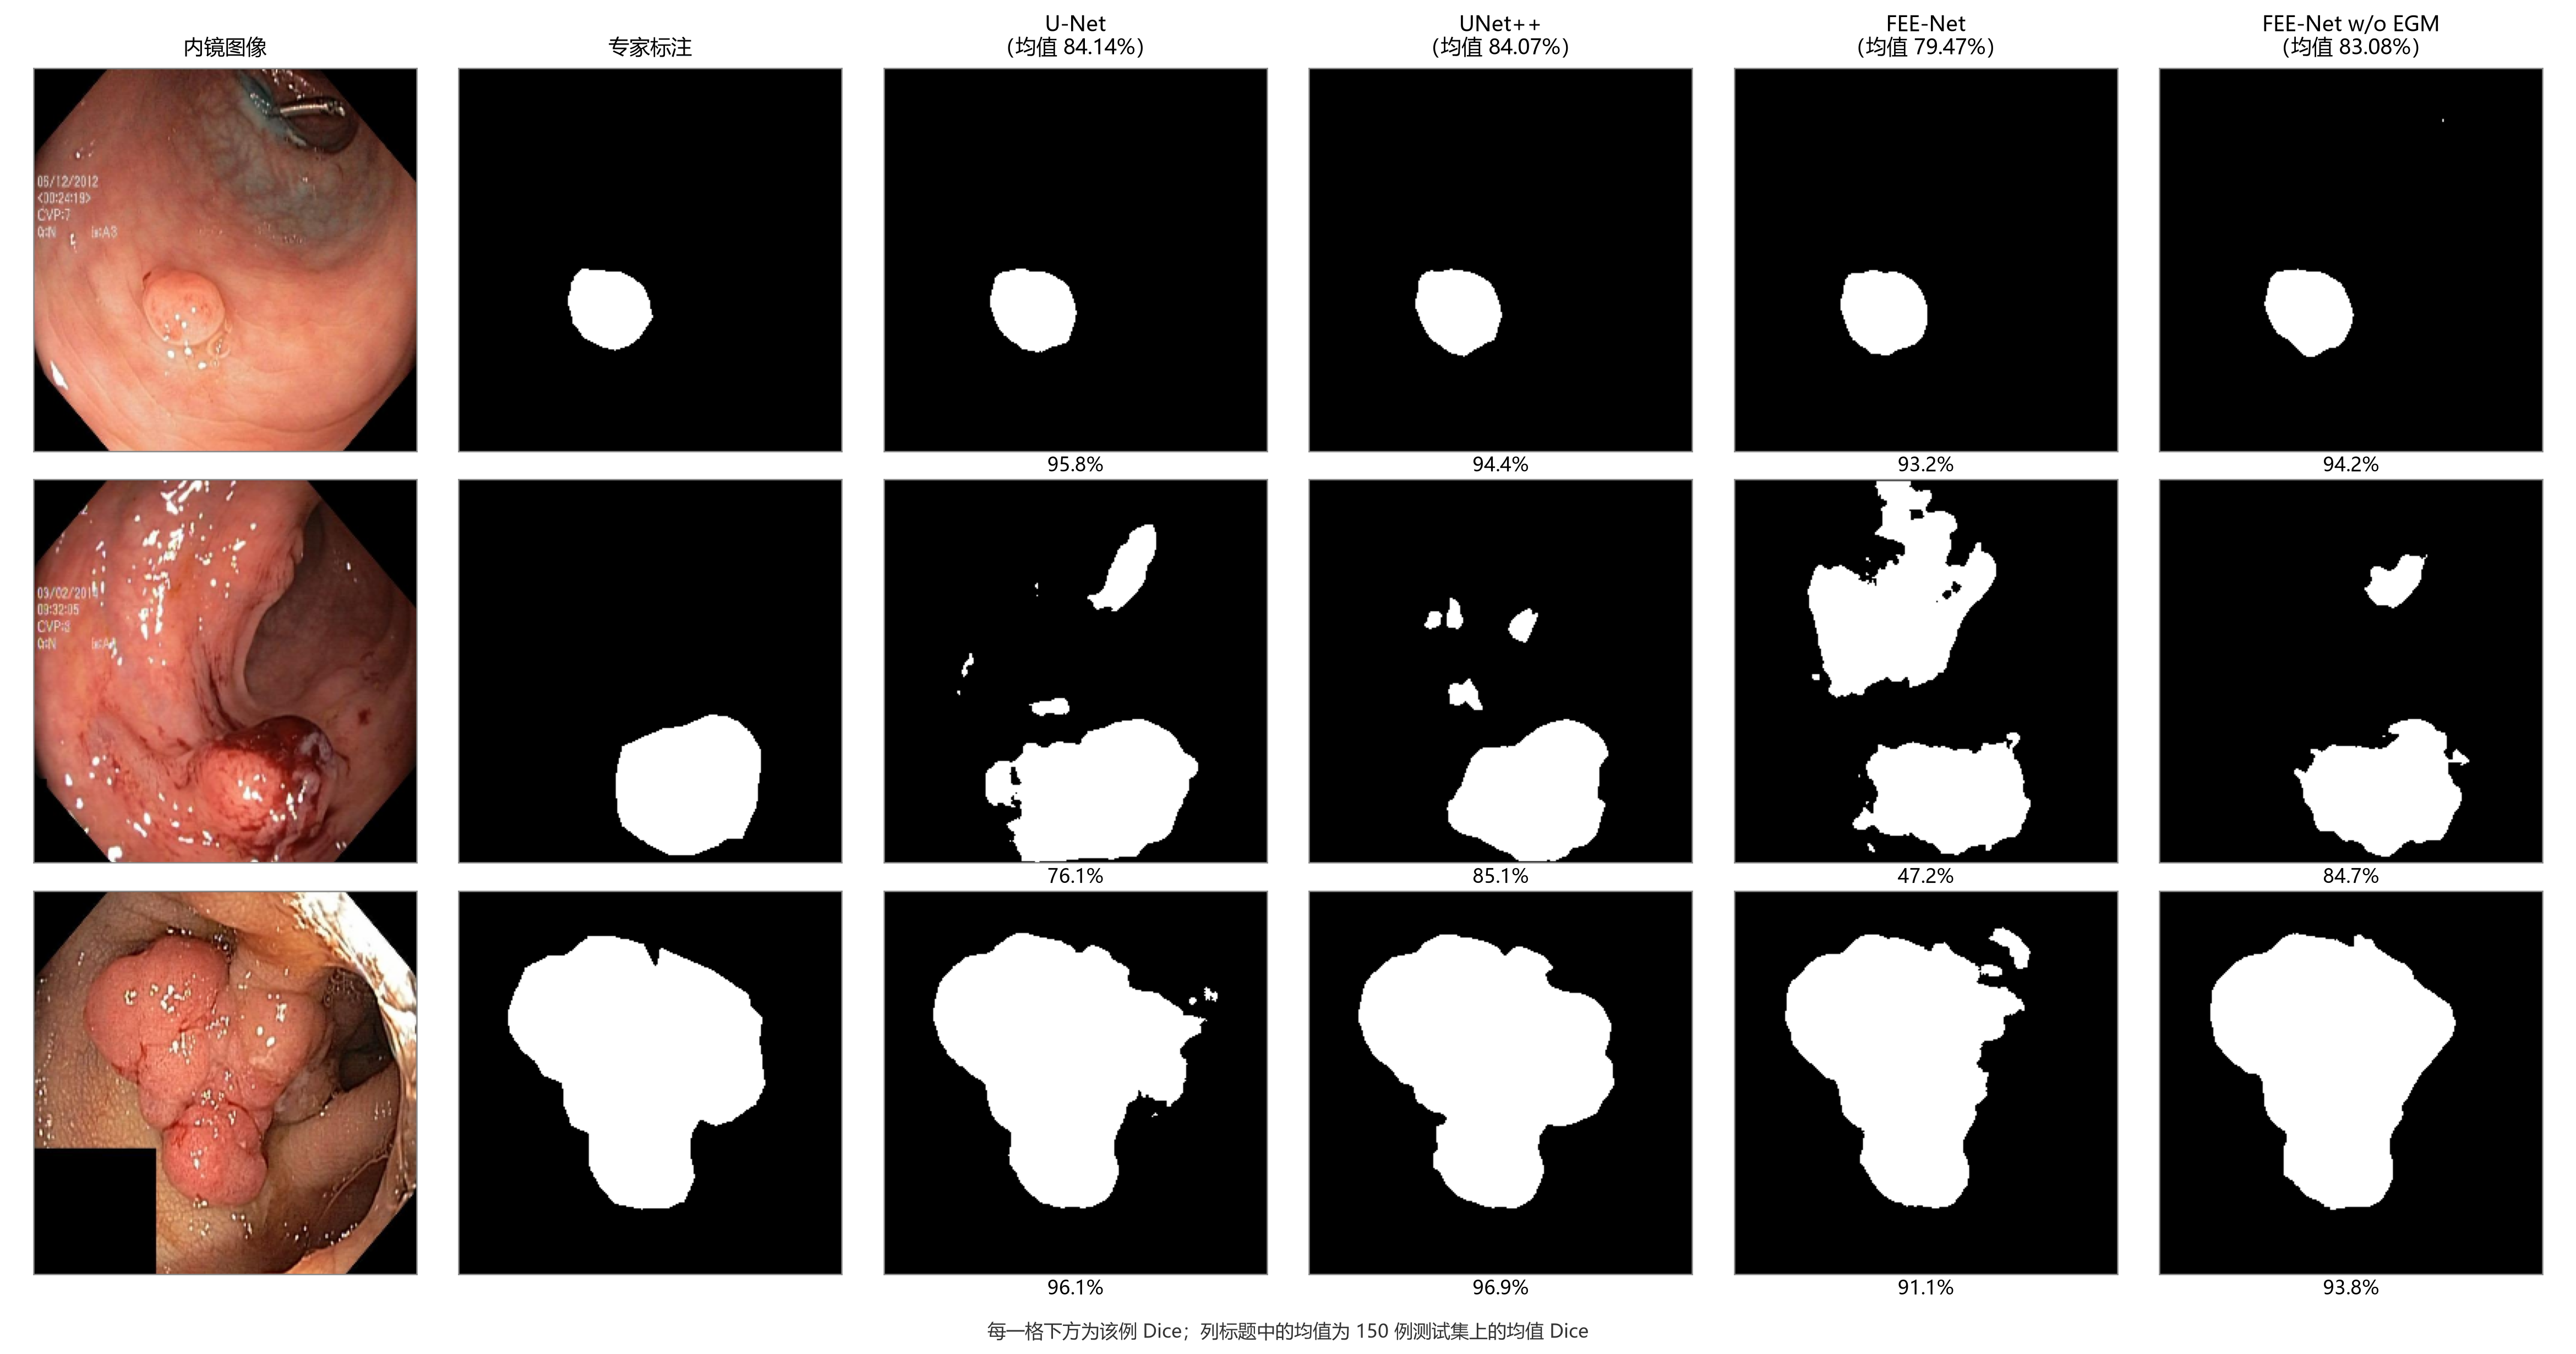
\includegraphics[width=0.98\textwidth]{figure_qualitative_v6.png}
\caption{留出测试帧上的定性表现。三行分别为 150 例测试帧中病灶面积的第 10、50、90 百分位（选取规则确定且可复现）。列标题中的均值为该配置在 150 例测试集上的均值 Dice，每格下方为该例 Dice。中间一例最能说明问题：完整 FEE-Net 在病灶周边产生大片假阳区域（该例 Dice 仅 47.2\%），而移除边缘门控模块后恢复到 84.7\%——这是第5.3 节“EGM 在 Dice 与边界误差上均有害”这一归因结论的直接可视证据。\\ Qualitative behaviour on held-out test frames. Rows are the 10th, 50th and 90th percentile of lesion area; column headers carry the mean test Dice of each configuration and the value under each panel is the per-case Dice.}
\label{fig:qual}
\end{figure*}

\subsection{组件归因：辅助损失有益，边缘门控模块有害}

表3在验证折上以 60 轮预算逐项隔离各训练项。移除深监督损失 2.86 个 Dice 点，移除边界 IoU 项损失 1.03，移除边缘 BCE 项损失 0.63；三项全去掉（仅 BCE 加 Dice）损失 2.95。单项惩罚之和为 4.52，故联合惩罚比各项之和小 1.57 点。一种合理的解读是三项作用于相互重叠的失效模式，但我们的设计并未直接检验该机制。无论机制如何，其实践后果成立：把单项增量相加的消融表会高估捆绑损失的价值，因此我们明确报告联合一行。

\begin{table}[t]
\centering

\caption{表3 验证折（170 帧，60 轮，同种子同日程）上的组件归因。增量为相对完整配置的差值。末行为同协议训练的朴素 U-Net，作参照而非消融。}
\label{tab:ablation}
\resizebox{\columnwidth}{!}{%
\begin{tabular}{lccc}
\toprule
\textbf{配置} & \textbf{验证 Dice (\%)} & \textbf{Δ Dice} & \textbf{验证 HD95 (px)} \\
\midrule
完整配置（五项全开） & 77.55 & — & 40.14 \\
去边界 IoU 项 & 76.52 & -1.03 & 43.28 \\
去边缘 BCE 项 & 76.92 & -0.63 & 45.81 \\
去深监督 & 74.69 & -2.86 & 50.21 \\
仅 BCE+Dice & 74.60 & -2.95 & 48.17 \\
U-Net，同协议 & 77.92 & +0.37 & 50.11 \\
\bottomrule
\end{tabular}}
\end{table}

架构消融的行为不同，且与设计依据相悖。移除离散小波前端损失 1.31 个 Dice 点（80.78 对 79.47），这对一个旨在保留高频结构的组件而言是预期方向。然而移除边缘门控模块反而获得 3.61 个 Dice 点（83.08 对 79.47），同时把 HD95 从 38.67 px 改善到 31.71 px，并把计算量从 12.59 降到 11.83 GFLOPs。换言之，那个支撑“边缘感知”这半个架构名的模块，是我们所测每一个轴上都明确有害的唯一组件。因此该族的推荐配置是 FEE-Net w/o EGM，而非 FEE-Net。

需要强调这与表3的损失各行并不矛盾：边缘 BCE 损失与边缘门控模块是两个不同的对象，我们的数据把它们清晰分开。对辅助边缘头施加监督能改善模型（表3）；而把高频响应经语义门控送入解码器则不能（表2）。

\subsection{边界保真度：频域路径在哪里兑现}

Dice 与豪斯多夫距离在我们的数据上明显解耦，而这种解耦是有信息量的。基线中 UNet++ 取得最好 HD95（33.38 px），尽管 Dice 与其余基线持平，这与其嵌套跳跃路径缩小语义差距的设计相符\cite{zhou2018unetpp}。FEE-Net 的 HD95（38.67 px）反而差于所有基线，说明频域路径本身并不自动带来边界精度。

组件证据表明边界信号确实存在，且归因正确。在探针中，移除边界 IoU 项使 HD95 由 40.14 退化到 43.28 px，即 3.14 px 的惩罚，而朴素 U-Net 参照为 50.11 px。该项使用的形态学带状区域，正是作为周长损失软轮廓提出的最大池化膨胀减最小池化腐蚀构造\cite{eljurdi2021perimeter}，也更早被用于通过差异图上的腐蚀直接优化豪斯多夫距离\cite{karimi2019hd}；同一带状构造构成 Boundary IoU 质量度量的基础\cite{cheng2021boundaryiou}。我们的贡献不是该算子，而是证明在本流水线中正是它承载了边界收益——并且该收益只在移除边缘门控模块后才能完全兑现：此时 HD95 达到 31.71 px，在全部七种配置中最低，较 U-Net（36.33 px）降低 12.7\%、较 Attention U-Net（38.73 px）降低 18.1\%、较最强的经典基线 UNet++（33.38 px）降低 5.0\%，而 Dice 仅比 U-Net 低 1.06 个百分点。换言之，本文架构的竞争力并不体现在区域重叠上，而体现在边界定位精度上——对息肉切除边界的界定而言，后者比 Dice 更具临床相关性。

\begin{figure}[t]
\centering
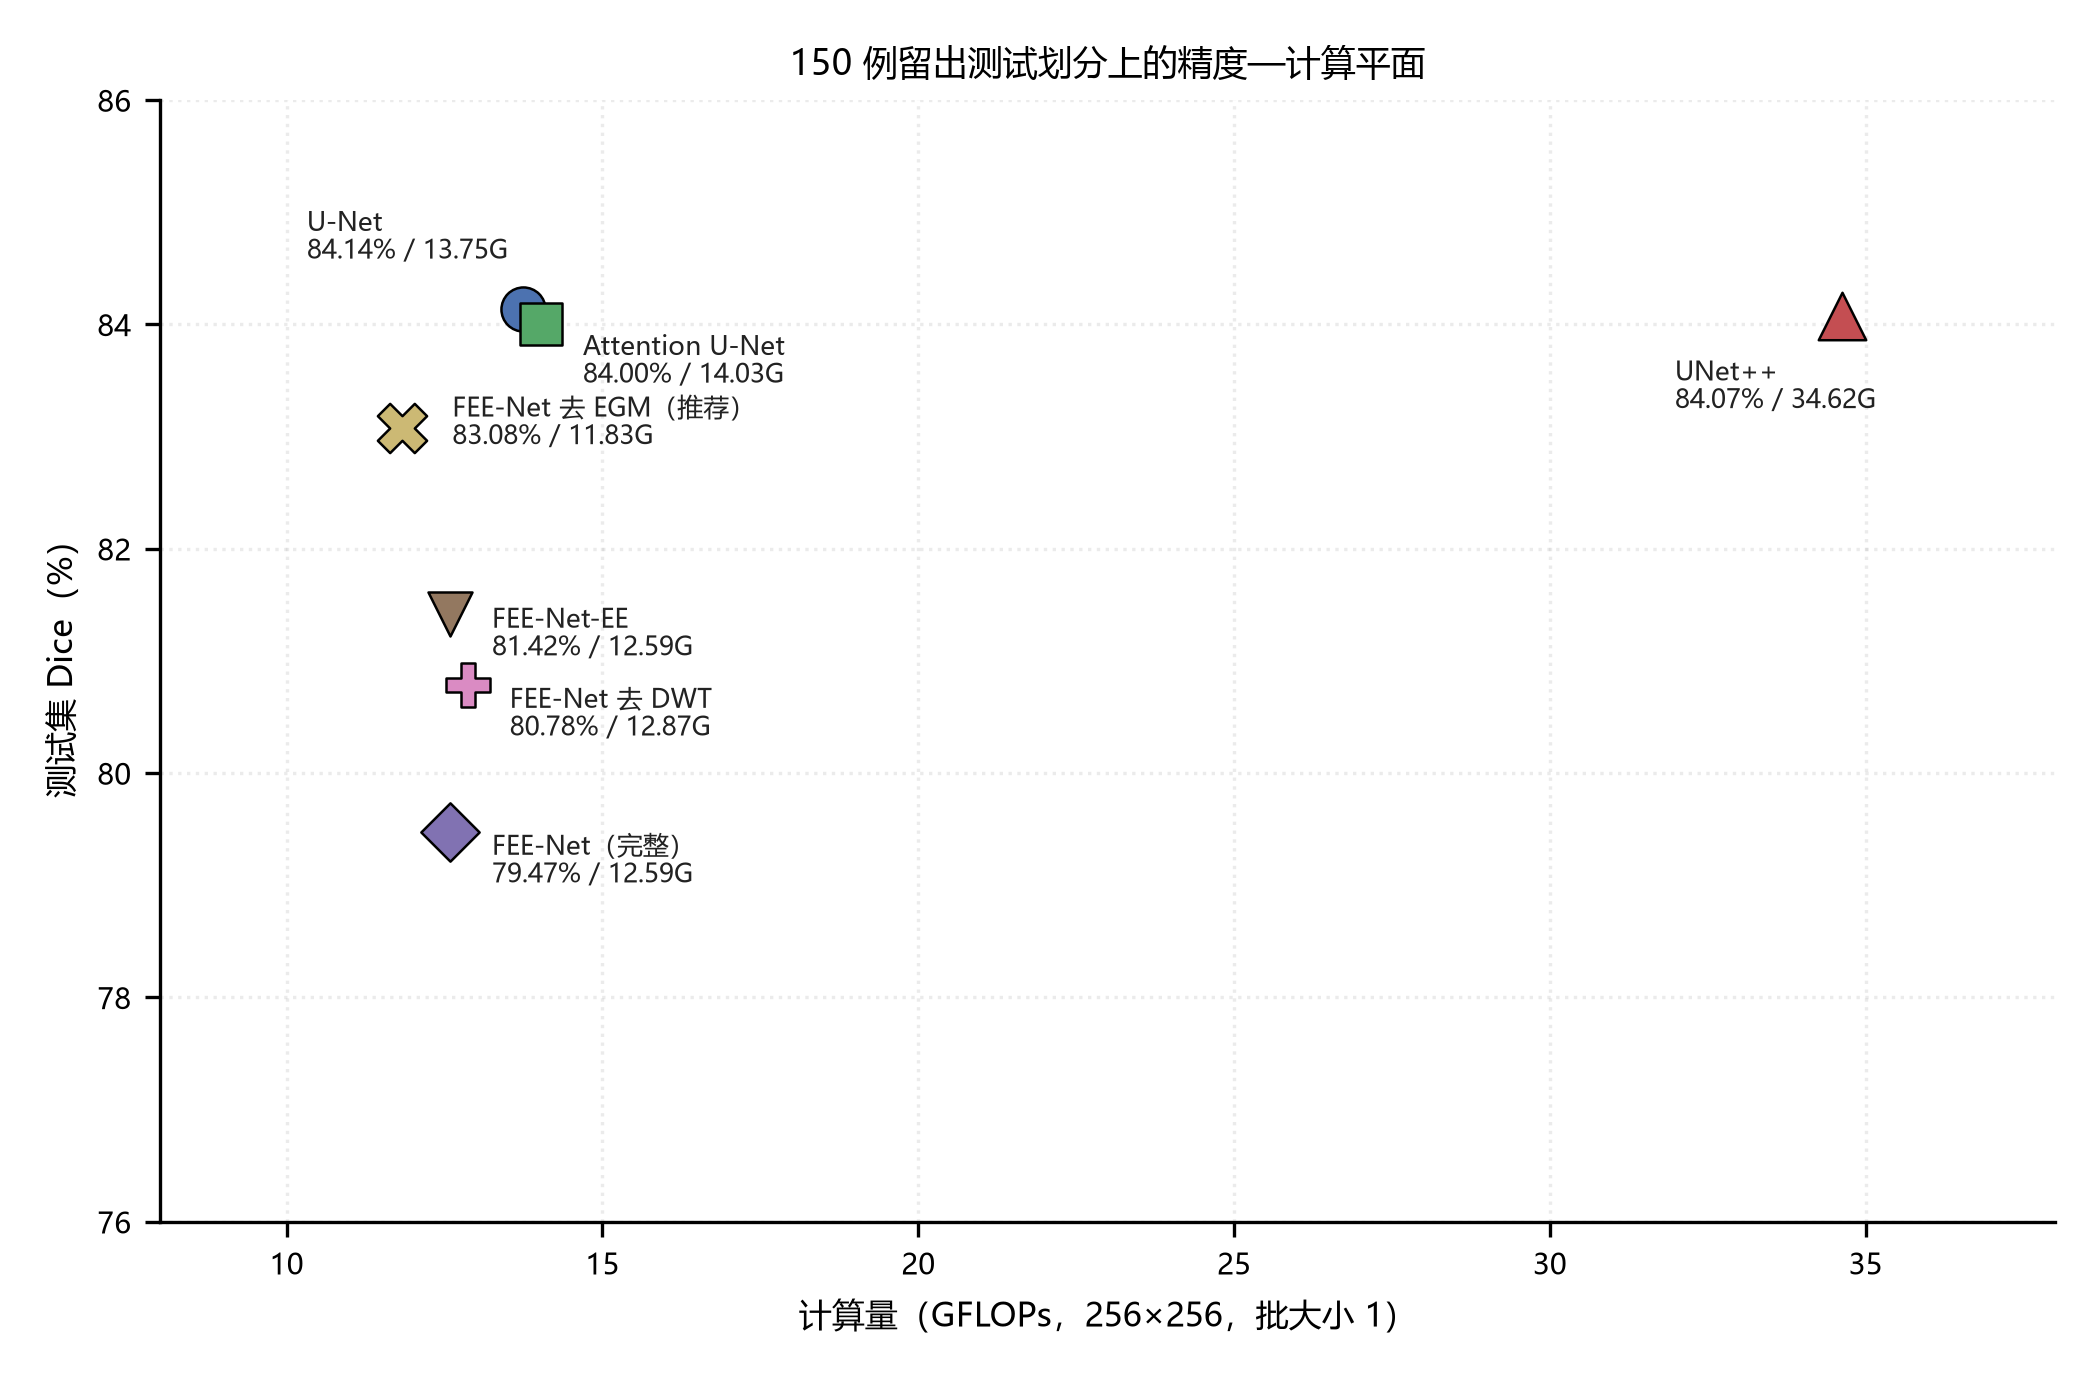
\includegraphics[width=0.96\columnwidth]{figure_pareto_v5_zh.png}
\caption{七种配置的精度—计算平面（各配置数值见表2），直接由基准 CSV 绘制。标记面积与 HD95 成反比。没有配置支配其他配置：基线聚集在约 84\% Dice、13.75–34.62 GFLOPs 处，而 FEE-Net w/o EGM 以 83.08\% Dice、11.83 GFLOPs 取得全文最低的边界误差。\\ Accuracy-computation plane for the seven configurations of Table 2, plotted directly from the benchmark CSV. Marker area scales inversely with HD95.}
\label{fig:pareto}
\end{figure}

\subsection{保形认证的分流级联与实测节省}

Kvasir-SEG 是全阳性集合——每一帧都含息肉——因此它本身无法量化筛查门正确跳过健康黏膜的频率，也无法量化由此节省的计算。我们因此仅用留出测试帧构建混合队列：病灶帧作为正样本，取自同一帧、且距标注病灶安全距离之外的黏膜裁剪作为负样本（第4.2 节）。该队列按排序序号交替拆分为互不共享帧的校准半（75 例病灶、134 例黏膜）与认证半（75 例病灶、133 例黏膜）。

分流头并未在该队列上训练。它分两阶段训练：分割主干作为基准的一部分在 fold-0 训练划分上训练一次，随后仅分流头（12 740 个参数）在一个独立的、分布匹配的均衡队列上微调，该队列由 fold-0 的训练与验证帧构建，且主干保持推理模式（第3.5 节）。校准与认证随后在未经触碰的测试派生队列上进行。

表4给出认证工作点。在 $\tau$* = 0.59 处，认证半中没有任何病灶帧被旁路（0/75），95\% 置信下精确 Clopper–Pearson 上界为 3.92\%，低于 5\% 目标。由于该上界是对 n = 75 时零事件的取值，它与闭式 1 - 0.05\textsuperscript{1/75} 相同；我们以该恒等式作为实现的单元校验。在同一阈值下，99.25\% 的无病灶黏膜裁剪被旁路，整个混合队列中 63.46\% 提前退出，实测延迟由完整路径的 11.30 ms 降到有效 5.93 ms，即 1.91 倍下降。

\begin{table}[t]
\centering

\caption{表4 保形认证的分流工作点。校准半与认证半在帧级互不相交。延迟以单台设备上的 CUDA 事件测量；门开销包含 stem、第一编码阶段、小波分支与分流头。}
\label{tab:triage}
\resizebox{\columnwidth}{!}{%
\begin{tabular}{lc}
\toprule
\textbf{量} & \textbf{数值} \\
\midrule
校准集（病灶 / 黏膜） & 75 / 134 \\
认证集（病灶 / 黏膜） & 75 / 133 \\
校准阈值 $\tau$* & 0.59 \\
Clopper–Pearson 上界（校准） & 3.92\% \\
实测 FNR（认证） & 0/75 = 0.00\% \\
Clopper–Pearson 上界（认证） & 3.92\% \\
无病灶黏膜旁路率 & 99.25\% \\
整个混合队列旁路率 & 63.46\% \\
分流门延迟 & 2.84 ms \\
完整路径延迟 & 11.30 ms \\
有效延迟 & 5.93 ms \\
实测加速比 & 1.91 倍 \\
\bottomrule
\end{tabular}}
\end{table}

工作曲线在关键区间异常平坦。当 $\tau$ 从 0.05 变到 0.40，认证 FNR 始终为 0.00\%，而黏膜旁路率仅从 98.50\% 变动到 99.25\%；当 $\tau$ 超过 0.70，才开始以出现首批漏诊为代价换取不到一个百分点的旁路率。对部署而言，平台区是理想性质，因为它意味着决策规则对校准估计的微小误差不敏感；但它同时意味着绝大部分可获得的节省在很低的阈值处就已经兑现，$\tau$* 的选择应由认证而非经验最优点决定。

\subsection{两个使朴素实现失效的陷阱}

以下两种失效都产生了看似合理的输出，且只有通过针对性检查才被发现。我们报告它们，因为二者都不为本架构所特有。

全阳性队列下的坍缩。我们最初的实现把分流头与分割在 fold-0 训练划分上联合训练——680 帧，全部含息肉。单类目标上的交叉熵存在平凡最优解：永远预测“病灶”。训练后的分流头对每一帧（无论病灶或黏膜）都输出 0.9998 的风险，于是旁路率为 0.00\%、实测加速为 1.0 倍，而假阴性率空洞地为 0。本工作的一个早期版本曾报告 64.66\% 的旁路率；我们现已追溯该数字，发现它来自一个被无关的验证缺陷冻结在坍缩之前的检查点，其病灶与黏膜的风险分离度仅为 0.012。该数字不可复现，已撤回。纠正配方即第3.5 节的两阶段日程：门必须在含负样本的队列上训练，且该队列须与部署分布匹配。

批归一化统计量透过冻结主干泄漏。第二种失效更隐蔽。以 requires\_grad=False 冻结共享主干只能阻止梯度回传，并不能阻止模块处于训练模式时批归一化的滑动统计量被更新。在我们最初的仅训头微调尝试中，所得模型的分割 Dice 从 81.42\% 跌到 14.06\%——这一灾难性退化没有任何训练损失会提示，因为该阶段从未优化分割头。把共享路径置为推理模式、仅训练分流头后，Dice 恢复到 81.42\%，与微调前逐位相同，同时保留了门的判别力。因此任何共享归一化主干的两阶段流水线，都必须显式断言模块模式，而不能依赖梯度冻结。

第三种较轻微的隐患值得记录，因为它会静默抬高表观性能：本项目早期基于完整 Kvasir-SEG 构建的辅助均衡队列中，含同时出现在留出测试划分里的帧（在我们核查的 480 张训练图中有 68 张、120 张验证图中有 24 张）。若不加过滤地在其上训练分流头，就会把测试帧泄漏进校准流水线。我们的构建器按源帧过滤，并断言与测试划分零重叠。

\section{讨论}

\subsection{主要发现}

四项发现组织了本研究。第一，在匹配协议下，一个复合频域架构未能超过朴素 U-Net：79.47\% 对 84.14\% Dice，而参数量多 10.0\%。该差距远大于我们在验证折上测得的 0.37 点差异（77.55 对 77.92）；我们把这一落差作为关于本队列的观察记录，而不作为关于验证协议的普遍结论，因为单一划分无法分离二者。

第二，本文架构的收益集中在边界而非区域重叠。三项辅助损失各自有益且联合呈次可加；移除在 Dice 与 HD95 上双重有害的边缘门控模块后，该族最佳配置达到 83.08\% Dice 与 31.71 px HD95——后者是全文最低的边界误差，较 U-Net 降低 12.7\%、较 UNet++ 降低 5.0\%，而 Dice 仅低 1.06 个百分点。由于息肉切除范围的判定依赖边界而非区域面积，这一取舍在临床上是有利的。

第三，认证级联是系统中真正带来部署相关收益的部分。在校准与认证于帧级分离的前提下，门旁路了 99.25\% 的无病灶黏膜，同时未漏掉 75 例认证病灶中的任何一例，精确上界 3.92\%，实测 1.91 倍延迟下降。该节省在绝对值上并不惊人，因为门本身耗时 2.84 ms，而完整路径为 11.30 ms；但它是实测且经认证的节省，而非外推值。

第四，我们记录的两个失效模式对常规监控均不可见。坍缩的门报告零假阴性；被污染的主干在其训练阶段报告健康的分割损失。因此这类系统的可保证性需要结构性检查——门训练队列的类别平衡、显式的模块模式断言、辅助数据的源帧过滤——而不仅是指标监控。

\subsection{与先前工作的关系}

频域息肉分割是一个活跃且拥挤的方向，本文结果应被读作警示而非竞争者。WRANet 以离散小波变换取代池化并去除高频以抑制噪声，在 CVC-ClinicDB 上报告 88.89\% Dice\cite{zhao2023wranet}。AdaptUNet 把小波前端与注意力 U-Net 结合，在 HyperKvasir 上训练后于 CVC-300 报告 0.9104 Dice\cite{rajasekar2024adaptunet}。MEGANet-W 向每个解码阶段注入免参数 Haar 小波边缘图，在五个息肉数据集上最高提升 1.2 mDice\cite{yeemeganet2025}。2026 年的跨频带框架通过融合 RGB 与灰度小波子带，在 Kvasir 上报告 0.885 mDice，论据是灰度在各细节频带上保持更高的边界对比度\cite{oh2026crossband}。作为边界感知基线的代表，PraNet 以反向注意力在 Kvasir 上报告 0.898 Dice\cite{fan2020pranet}。

表5把这些数字与本文结果并列，并显式标注其评测设置。该比较刻意不是排序：已发表数值来自同一名义数据集的不同划分、不同输入分辨率与不同训练预算，且在若干情形下其训练集是所报测试集的超集。我们自己的 U-Net 参照在本 150 帧划分上达到 84.14\%，低于 PraNet 在 80/10/10 随机划分下报告的 89.8\%\cite{fan2020pranet}；我们并不把这一差异解读为架构裁决，因为划分不同、预算不匹配。这正是促使我们开展本次审计的可比性问题。

\begin{table}[t]
\centering

\caption{表5 频域与边界感知文献中报告的息肉分割精度，并标注其评测设置。各行之值不可直接比较（划分、分辨率与预算均不同），列出它们是为了让这种不可比性显式化，而非用于排名。}
\label{tab:literature}
\resizebox{\columnwidth}{!}{%
\begin{tabular}{lccc}
\toprule
\textbf{方法} & \textbf{出处} & \textbf{评测集} & \textbf{Dice} \\
\midrule
WRANet \cite{zhao2023wranet} & Complex Intell. Syst. 2023 & CVC-ClinicDB & 88.89 \\
AdaptUNet \cite{rajasekar2024adaptunet} & Heliyon 2024 & CVC-300 & 91.04 \\
MEGANet-W \cite{yeemeganet2025} & arXiv 2025 & 五个息肉集 & +1.2 mDice \\
跨频带 \cite{oh2026crossband} & arXiv 2026 & Kvasir & 88.5 \\
PraNet \cite{fan2020pranet} & MICCAI 2020 & Kvasir（80/10/10） & 89.8 \\
PrysmNet \cite{xiao2026prysmnet} & npj Digit. Med. 2026 & 同中心区间 & 85–95 \\
U-Net（本审计） & — & Kvasir-SEG，150 留出 & 84.14 \\
FEE-Net w/o EGM & — & Kvasir-SEG，150 留出 & 83.08 \\
\bottomrule
\end{tabular}}
\end{table}

在统计一侧，我们的级联是对若干已成熟思想的直接应用：以风险控制预测集对一般损失给出分布无关的有限样本控制\cite{bates2021rcps}，以保形风险控制处理单调损失且保守性至多 O(1/n)\cite{angelopoulos2022crc}，以及在可交换性下成立的分裂保形\cite{angelopoulos2021gentle}。医学应用推进迅速：CLS 校准逐扫描阈值，使测试期假阴性率低于给定容差\cite{tan2025cls}；保形风险控制也被用于管理医学实例分割的错误发现率\cite{dai2025crcfdr}。我们的贡献不在机制本身，而在其落点：一个帧级的分流决策，在无泄漏混合队列的一半上校准、在另一半上一次性认证，并把实测率与上界并列报告、把实际耗时而非外推值作为节省依据。2026 年的 PET/CT 研究是对任何乐观的必要制衡：全局阈值无法在 $\alpha$=$\delta$=0.1 下认证二值漏诊损失，因为即便取所评估的最小阈值，校准集经验风险仍为 0.177，作者正确地将其诊断为预测族的支撑失败，而非保形风险控制的失败\cite{zheng2026crc}。我们的认证在 5\% 目标、n = 75 下成立；若目标收紧到 1\%，则需要约四倍数量的校准病灶，因此我们并不把它当作“任何漏诊损失均可认证”的证据。

\subsection{对部署的启示}

三点实践启示。第一，报告一个脱离划分与预算的分割 Dice 几乎不具信息量；我们测得的两个架构之间 4.67 点的差距，小于我们的 U-Net 与 PraNet 已发表数值之间的差距，而后者是协议假象。第二，组件消融对多组件设计应成为强制项，并且必须允许出现“某组件有害”的结论——我们的边缘门控模块通过了设计评审、实现与完整训练，只在单分支消融下才被击落。第三，筛查门应由其认证来规定，而非由其工作曲线来规定：曲线说明节省在哪里，认证说明该节省是否可被采纳。

\subsection{局限性}

单划分、单种子。表2至表4中的每个数字都是单次划分、单一种子下的点估计。我们不为 Dice 报告置信区间，也不作显著性声明，因为那需要重复训练，而本研究未进行。仓库提供了五折划分定义以便重复；在重复完成之前，表2的排序应被视为描述性的。

替代性负样本。混合队列中的“无病灶”类取自含息肉帧的黏膜裁剪，而非来自真正无息肉的检查帧。这使队列相对于测试划分无泄漏，但并未复现真实筛查流的表观分布——在真实筛查流中，正常帧来自不同患者与不同采集语境。因此 99.25\% 的旁路率应被读作部署门可达性能的上界。

单一硬件平台。延迟与 FPS 在单台设备上测量；绝对值以及由此得到的 1.91 倍加速在其他硬件上会不同。比值比绝对延迟更可移植，因为分子与分母在同一设备、同一时段测得，但我们不主张跨平台有效性。

认证范围。该保证假设校准半与认证半之间可交换。两半均来自同一数据集同一 150 帧划分，因此认证不跨中心、跨扫描仪或跨肠道准备方案迁移；文献记录的 15.1\% 泛化落差正是对该保证的直接威胁\cite{divya2026review}。要把认证扩展到发生偏移的人群，需要加权保形校准或在部署现场重新校准。

单一数据集。我们仅在 Kvasir-SEG 上评测。跨数据集行为——即该领域已报告 Dice 崩塌到 0.6–0.7 之处\cite{xiao2026prysmnet}——在本文中未被检验。

\section{结论}

我们在无泄漏协议下审计了一个频域边缘感知息肉分割器，隔离了它的组件，并对其筛查门做了认证。审计给出一个负面的架构结论——该复合设计落后朴素 U-Net 4.67 个 Dice 点，且其边缘门控模块在每个轴上都为负——一个正面的边界结论——推荐配置以 31.71 px 的 HD95 取得全场最优的边界定位精度，较 U-Net 降低 12.7\%——以及一个正面的系统结论：在无泄漏混合队列互不相交的两半上分别校准与认证的分流级联，以 3.92\% 的精确上界旁路了 99.25\% 的无病灶黏膜，并带来实测 1.91 倍的延迟下降。其间我们识别出两个静默失效模式：全阳性的门训练队列使其坍缩为常数输出，批归一化泄漏则摧毁被冻结的主干；二者都能穿过常规指标监控而不被察觉。

更一般的教训是：息肉分割当前缺的不是精度，而是保证。同中心 Dice 0.85–0.95 与跨中心 0.6–0.7 并存，而一个通过了设计评审、实现与完整训练的组件，仍然可能值得被移除。隔离测试划分的协议、允许返回否定答案的消融、以及附带有限样本认证的工作点，在我们看来是从已发表的最新水平走向结肠镜室可以依赖之物的一条最短路径。

\section{数据与代码可用性}

Kvasir-SEG 公开可用。划分定义、基准生成器、混合队列构建器、分流头微调脚本与认证脚本随本文发布，并附含本次报告运行所用确切源文件的溯源包。

\begin{thebibliography}{99}
\bibitem{divya2026review}
DIVYA D S, SUDHA M. Deep learning driven colorectal polyp analysis: a review of detection, classification and segmentation methods[J]. Frontiers in Artificial Intelligence, 2026, 9. DOI: 10.3389/frai.2026.1786679.

\bibitem{xiao2026prysmnet}
XIAO J, HAN Y, WANG L, et al. PrysmNet: a polyp refining system using salience and multimodal guidance for reproducible cross domain segmentation[J]. npj Digital Medicine, 2026, 9. DOI: 10.1038/s41746-026-02345-7.

\bibitem{jha2020kvasir}
JHA D, SMEDSRUD P H, RIEGLER M A, et al. Kvasir-SEG: a segmented polyp dataset[C]//Proceedings of the International Conference on Multimedia Modeling (MMM). 2020: 451-462.

\bibitem{ali2023polypgen}
ALI S, JHA D, GHATWARY N, et al. PolypGen: a multi-center polyp detection and segmentation dataset for generalisability assessment[J]. Scientific Data, 2023, 10: 75.

\bibitem{chen2021transunet}
CHEN J, LU Y, YU Q, et al. TransUNet: transformers make strong encoders for medical image segmentation[EB/OL]. (2021). https://arxiv.org/abs/2102.04306.

\bibitem{ruan2024vmunet}
RUAN J, LI J, XIANG S. VM-UNet: vision Mamba UNet for medical image segmentation[EB/OL]. (2024). https://arxiv.org/abs/2402.02491.

\bibitem{ma2024medsam}
MA J, HE Y, LI F, et al. Segment anything in medical images[J]. Nature Communications, 2024, 15: 654.

\bibitem{zhao2023wranet}
ZHAO Y, WANG S, ZHANG Y, et al. WRANet: wavelet integrated residual attention U-Net network for medical image segmentation[J]. Complex \& Intelligent Systems, 2023, 9(6): 6971-6983.

\bibitem{rajasekar2024adaptunet}
RAJASEKAR D, THEJA G, PRUSTY M R, et al. Efficient colorectal polyp segmentation using wavelet transformation and AdaptUNet: a hybrid U-Net[J]. Heliyon, 2024, 10(13): e33655.

\bibitem{yeemeganet2025}
YEE T Z, QASEM A. MEGANet-W: a wavelet-driven edge-guided attention framework for weak boundary polyp detection[EB/OL]. (2025). https://arxiv.org/abs/2507.02668.

\bibitem{oh2026crossband}
OH H, LEE J. Polyp segmentation using wavelet-based cross-band integration for enhanced boundary representation[EB/OL]. (2026). https://arxiv.org/abs/2603.03682.

\bibitem{laskaridis2021earlyexit}
LASKARIDIS S, KOURIS A, LANE N D. Adaptive inference through early-exit networks: design, challenges and directions[C]//Proceedings of the International Workshop on Embedded and Mobile Deep Learning (EMDL). 2021.

\bibitem{demir2024earlyexit}
DEMIR E, AKBAS E. Early-exit convolutional neural networks[EB/OL]. (2024). https://arxiv.org/abs/2409.05336.

\bibitem{bates2021rcps}
BATES S, ANGELOPOULOS A, LEI L, et al. Distribution-free, risk-controlling prediction sets[J]. Journal of the ACM, 2021, 68(6): 1-34.

\bibitem{angelopoulos2022crc}
ANGELOPOULOS A N, BATES S, FISCH A, et al. Conformal risk control[C]//Proceedings of the International Conference on Learning Representations (ICLR). 2024.

\bibitem{angelopoulos2021gentle}
ANGELOPOULOS A N, BATES S. A gentle introduction to conformal prediction and distribution-free uncertainty quantification[EB/OL]. (2021). https://arxiv.org/abs/2107.07511.

\bibitem{tan2025cls}
TAN B, WANG Z, DUAN J, et al. Conformal lesion segmentation for 3D medical images[EB/OL]. (2025). https://arxiv.org/abs/2510.17897.

\bibitem{dai2025crcfdr}
DAI M, LUO W, LI T. Statistical management of the false discovery rate in medical instance segmentation based on conformal risk control[C]//Proceedings of the IEEE International Conference on Image Processing and Computer Applications (ICIPCA). 2025.

\bibitem{zheng2026crc}
ZHENG W, et al. What can conformal risk control certify for PET/CT tumour segmentation?[C]//Proceedings of the Conference on Conformal and Probabilistic Prediction with Applications. PMLR, 2026, 329: 1-3.

\bibitem{ronneberger2015unet}
RONNEBERGER O, FISCHER P, BROX T. U-Net: convolutional networks for biomedical image segmentation[C]//Proceedings of the International Conference on Medical Image Computing and Computer-Assisted Intervention (MICCAI). 2015: 234-241.

\bibitem{zhou2018unetpp}
ZHOU Z, RAHMAN SIDDIQUEE M M, TAJBAKHSH N, et al. UNet++: a nested U-Net architecture for medical image segmentation[C]//Proceedings of the MICCAI Deep Learning in Medical Image Analysis Workshop. 2018: 3-11.

\bibitem{oktay2018attention}
OKTAY O, SCHLEMPER J, LE FOLGOC L, et al. Attention U-Net: learning where to look for the pancreas[C]//Proceedings of the International Conference on Medical Imaging with Deep Learning (MIDL). 2018.

\bibitem{fan2020pranet}
FAN D P, JI G P, ZHOU T, et al. PraNet: parallel reverse attention network for polyp segmentation[C]//Proceedings of the International Conference on Medical Image Computing and Computer-Assisted Intervention (MICCAI). 2020: 263-273.

\bibitem{hu2018senet}
HU J, SHEN L, SUN G. Squeeze-and-excitation networks[C]//Proceedings of the IEEE/CVF Conference on Computer Vision and Pattern Recognition (CVPR). 2018: 7132-7141.

\bibitem{qin2021fcanet}
QIN Z, ZHANG P, WU F, et al. FcaNet: frequency channel attention networks[C]//Proceedings of the IEEE/CVF International Conference on Computer Vision (ICCV). 2021: 783-792.

\bibitem{karimi2019hd}
KARIMI D, SALCUDEAN S E. Reducing the Hausdorff distance in medical image segmentation with convolutional neural networks[J]. IEEE Transactions on Medical Imaging, 2020, 39(2): 499-513.

\bibitem{eljurdi2021perimeter}
EL JURDI R, PETITJEAN C, HONEINE P, et al. A surprisingly effective perimeter-based loss for medical image segmentation[C]//Proceedings of Medical Imaging with Deep Learning (MIDL). PMLR, 2021, 143: 158-167.

\bibitem{cheng2021boundaryiou}
CHENG B, GIRSHICK R, DOLLAR P, et al. Boundary IoU: improving object-centric image segmentation evaluation[C]//Proceedings of the IEEE/CVF Conference on Computer Vision and Pattern Recognition (CVPR). 2021: 15334-15342.

\bibitem{milletari2016vnet}
MILLETARI F, NAVAB N, AHMADI S A. V-Net: fully convolutional neural networks for volumetric medical image segmentation[C]//Proceedings of the International Conference on 3D Vision (3DV). 2016: 565-571.

\bibitem{lee2015dsn}
LEE C Y, XIE S, GALLAGHER P, et al. Deeply-supervised nets[C]//Proceedings of the International Conference on Artificial Intelligence and Statistics (AISTATS). PMLR, 2015, 38: 562-570.

\bibitem{odena2016checker}
ODENA A, DUMOULIN V, OLAH C. Deconvolution and checkerboard artifacts[EB/OL]. Distill, 2016. DOI: 10.23915/distill.00003.

\bibitem{clopper1934}
CLOPPER C J, PEARSON E S. The use of confidence or fiducial limits illustrated in the case of the binomial[J]. Biometrika, 1934, 26(4): 404-413.

\end{thebibliography}

\end{document}
